\documentclass[11pt,a4paper]{article}
\usepackage[margin=1in]{geometry}
\usepackage[hidelinks]{hyperref}
\usepackage{enumitem}
\usepackage{graphicx}
\usepackage{xcolor}
\usepackage{booktabs}
\usepackage{array}
\usepackage{longtable}
\usepackage{float}
\usepackage{caption}
\usepackage{needspace}
\graphicspath{{./}}

\widowpenalty=10000
\clubpenalty=10000
\raggedbottom

\makeatletter \newcommand{\BvrSetLabInstructor}[1]{\gdef\Bvr@LabInstructor{#1}}
\newcommand{\Bvr@LabInstructor}{Dr. Raghav B. Venkataramaiyer}
\newcommand{\BvrLabInstructorValue}{\Bvr@LabInstructor}
\makeatother

\usepackage{titling}
\setlength{\droptitle}{-5em}
\pretitle{\begin{center}\bfseries\fontsize{18bp}{18bp}\selectfont}
\makeatletter
\newcommand{\BvrSubtitle}[1]{
  \posttitle{
    \par\end{center}
    \begin{center}\large#1\end{center}
    \vskip 0.3em}
}
\makeatother

\newcommand{\BvrHint}[1]{{\normalfont\normalsize\itshape\hfill #1}}

\title{Campus Connect - A Closed-Community Social \& Academic Networking Platform}

\BvrSetLabInstructor{Dr. Jeelani Asif}

\BvrSubtitle{
  Project Proposal for UCS503 \\
  Submitted to: \BvrLabInstructorValue \\ \bfseries
  Thapar Institute of Engineering and Technology
}

\author{
  \begin{tabular}[t]{c}
    Prakhar Saxena, CSED \\
    {\small Roll No: 1024240019} \\
    {\small \nolinkurl{psaxena_be24@thapar.edu}}
  \end{tabular}
  \and
  \begin{tabular}[t]{c}
    Aayushmaan Singh Meyan, CSED \\
    {\small Roll No: 1024240142} \\
    {\small \nolinkurl{ameyan_be24@thapar.edu}}
  \end{tabular}
  \and
  \begin{tabular}[t]{c}
    Divyansh Jasrotia, CSED \\
    {\small Roll No: 1024240008} \\
    {\small \nolinkurl{djasrotia_be24@thapar.edu}}
  \end{tabular}
}

\predate{\begin{center}\small}\postdate{\end{center}\vspace{-0.5em}}
\date{August 15, 2026}

\begin{document}
\maketitle

\Needspace{5\baselineskip}
\section{Higher-Order Goal\BvrHint{\ldots secondary framing}}

This project aims to provide colleges, schools, and organisations with a private, verified, and structured digital environment that consolidates social networking and academic management into a single platform. The broader goal is to eliminate the fragmentation caused by using general-purpose public platforms for institutional communication, and to replace it with a purposeful, role-aware, and AI-safeguarded community space that serves students, teachers, and administrators alike.

\Needspace{5\baselineskip}
\section{Time-to-Value\BvrHint{\ldots primary heuristic}}
\begin{itemize}[leftmargin=0.7cm]
    \item Meaningful increments will be delivered by the end of each weekly sprint, beginning with core authentication and profile features and advancing to real-time communication and AI moderation.
    \item Fast feedback is prioritised over perfection: each completed module will be reviewed (and, where possible, CI-backed) before the next phase begins.
    \item Success in the first iteration is defined by a working login, profile, and social feed - enough for a real user to sign in, post, and connect.
\end{itemize}

\Needspace{5\baselineskip}
\section{Problem Statement}

Educational institutions and closed organisations currently face the following challenges when communicating and collaborating digitally:

\begin{itemize}[leftmargin=0.7cm]
    \item \textbf{No dedicated platform:} Colleges and schools rely on scattered public apps - WhatsApp groups, Instagram, and email chains - that are not designed for institutional or academic use.
    \item \textbf{Information gets lost:} Course materials, exam schedules, and placement updates are drowned in irrelevant personal content on general social media.
    \item \textbf{No internal trusted network:} Students and faculty have no way to build a verified, private network within their own community.
    \item \textbf{No access control:} Public platforms cannot restrict membership to verified community members only.
    \item \textbf{No content safety layer:} Institutions have no mechanism to detect or remove inappropriate, vulgar, or policy-violating content posted by members.
    \item \textbf{Fragmented communication:} Academic tools (timetables, assignments, resources) and social communication exist in completely separate, unconnected applications.
\end{itemize}

\textbf{Why this matters now (contextual relevance):} These inefficiencies lead to missed deadlines, lost resources, poor academic coordination, and an unsafe communication environment - all of which directly impact student performance and institutional effectiveness.

\Needspace{5\baselineskip}
\section{Proposed Solution\BvrHint{\ldots Software Proposition}}

\subsection{Overview}

Build a \textbf{web-based} closed-community social and academic networking platform with the following components:
\begin{itemize}[leftmargin=0.7cm]
    \item \textbf{Private and verified access:} only approved, verified members can join a community instance; admins control the join policy.
    \item \textbf{Social communication:} a structured social feed, friend system, direct messaging, and real-time notifications.
    \item \textbf{Academic utility:} a course materials hub, shared schedule board, and evaluation tracker for teachers and students.
    \item \textbf{Admin safety and control:} a full admin panel with user management, access control, content moderation, and an AI agentic moderation layer.
\end{itemize}

\subsection{System Architecture Overview}

Figure~\ref{fig:architecture} illustrates the proposed three-layer architecture of the platform.

\begin{figure}[H]
  \centering
  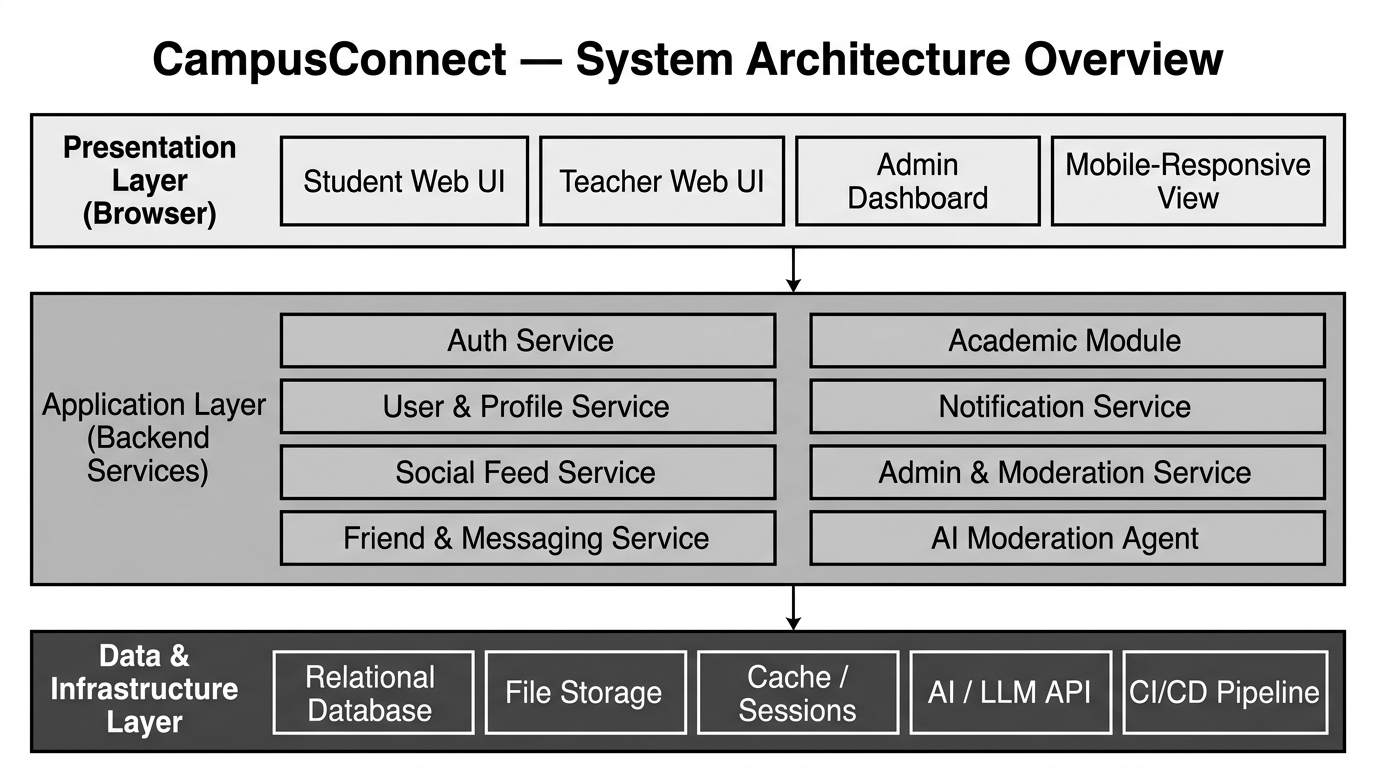
\includegraphics[width=0.9\textwidth]{CampusConnect_Architecture_BW.jpg}
  \caption{CampusConnect - Proposed System Architecture (Presentation, Application, and Data \& Infrastructure layers)}
  \label{fig:architecture}
\end{figure}

\subsection{Core Workflow}
\begin{enumerate}[leftmargin=0.7cm]
    \item Admin creates a community instance, sets the join policy, and adds the first users.
    \item Users sign up via institutional email or invite link, complete email verification, and set up their profile.
    \item Students join batch, lab, or subject groups; access course materials and the schedule board.
    \item Teachers publish lectures, exams, and evaluations on the group calendar and upload course resources.
    \item Members post in the social feed, connect as friends, and communicate via direct messages.
    \item Every post or comment is scanned by the AI moderation agent; flagged content is hidden and queued for admin review.
\end{enumerate}

\subsection{Operational Constraints for an Educational Setting}
\begin{itemize}[leftmargin=0.7cm]
    \item Fully browser-based - no app installation required; responsive design usable on desktops, tablets, and smartphones.
    \item Avoid dependence on advanced research algorithms; focus on workflow, automation, and system correctness.
    \item Designed for deployment on standard managed hosting and cloud database services.
\end{itemize}

\Needspace{5\baselineskip}
\section{Features and Functions\BvrHint{\ldots module breakdown}}

The platform is structured into eleven functional modules, each solving a specific institutional problem. This is an engineering course project, so the emphasis below is on scalable administrative and workflow design rather than novel algorithm research.

Figure~\ref{fig:modules} provides a visual overview of the primary functional modules.

\begin{figure}[H]
  \centering
  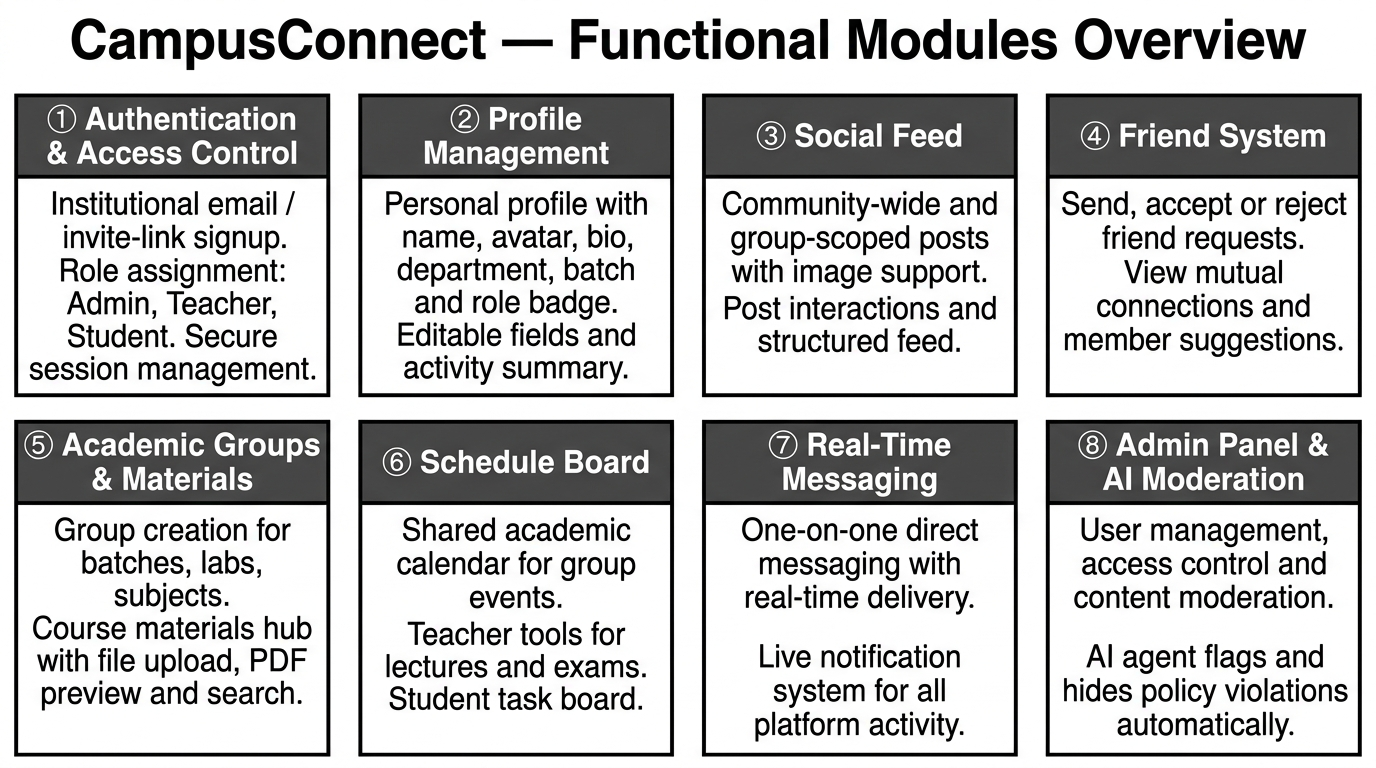
\includegraphics[width=0.92\textwidth]{CampusConnect_Modules_BW.jpg}
  \caption{CampusConnect - Functional Modules Overview}
  \label{fig:modules}
\end{figure}

\subsection{Authentication and Access Control}
Users will register using their institutional email or an admin-generated invite link. Email verification will confirm identity. The system will support role assignment (Admin, Teacher, Student), domain whitelisting, invite-link expiry control, and secure session management with password reset.

\subsection{Profile Management}
Every member will receive a personal profile page displaying their name, avatar, bio, department, batch, and role badge. Users will be able to edit all profile fields at any time. The profile will also show an activity summary of posts made, groups joined, and materials uploaded.

\subsection{Social Feed}
Members will create posts with text and image attachments. Posts will be scopable to the full community or to a specific group. Interactions will include likes and comments. The feed will aggregate content from friends and joined groups in a structured order. Authors and admins will be able to delete any post.

\subsection{Friend System}
Users will send, accept, or reject friend requests. They will be able to remove connections, view a full friends list, see pending requests, and receive suggestions based on shared batch, department, or mutual friends.

\subsection{Academic Groups}
Admins and teachers will create groups for batches, labs, subjects, or clubs. Students will browse and join open groups or accept invites. Each group will have its own feed, a materials section, and a schedule board. Group admins will be able to manage member roles and remove members as needed.

\subsection{Course Materials Hub}
Teachers and students will upload PDFs, notes, images, and external links, organised into subject or topic folders within each group. Members will be able to preview PDFs in-browser, download files, and search materials by name, subject, or uploader. An upload history log will track all contributions.

\subsection{Schedule Board}
A shared calendar will be available at the group level. Teachers will add lectures, exams, and evaluation deadlines. Students will add personal tasks and reminders visible only to themselves. Events will be colour-coded by type. A notification will be triggered whenever a new event is added to a group calendar.

\subsection{Direct Messaging}
Members will exchange real-time private messages. Messages will be delivered via WebSockets, support image attachments, and display delivery status. Users will have an inbox with unread badge counts and in-conversation search.

\subsection{Notifications}
A real-time notification bell will cover all platform activity: friend requests, post likes and comments, new messages, group invitations, and schedule events. Notifications will be markable as read individually or all at once, and each will link directly to the relevant content.

\subsection{Admin Module}

\textbf{User Management:} The admin will view all members in a table with role, status, and join date. Actions will include verifying new accounts, suspending or permanently removing members, changing roles, and bulk operations on multiple users.

\textbf{Access Control:} The admin will set the platform join policy as Open, Domain-Restricted, or Invite-Only. Invite links will be generated with configurable expiry dates and usage limits and can be revoked at any time. Email domain whitelisting will enforce institutional boundaries.

\textbf{Content Moderation:} The admin will review AI-flagged content in a dedicated queue, manually flag or remove any post or account, and view a full audit log of all moderation actions. Members will be able to submit post reports that appear in the admin dashboard.

\subsection{AI Agentic Content Moderation}
Every post and comment will be automatically scanned by an AI agent immediately upon submission. The agent will detect vulgarity, hate speech, harassment, and policy violations. Flagged content will be auto-hidden from the feed and the admin will be notified with a written justification for the flag. Admins will approve or permanently remove flagged content. A sensitivity control (Strict, Moderate, Lenient) and a global on/off toggle will be available in the admin settings; the AI layer will flag for human review rather than permanently deleting accounts autonomously.

\Needspace{5\baselineskip}
\section{Solution Approach\BvrHint{\ldots Engineering focus}}

\subsection{Tech Stack}
\begin{longtable}{>{\bfseries}p{4.5cm} p{8.5cm}}
\toprule
Component & Candidate Technology / Approach \\
\midrule
\endhead
Frontend Framework & Next.js (React, App Router) \\
Language & TypeScript \\
Styling & Tailwind CSS \\
Backend / API & Next.js API Routes (Node.js) \\
Database & PostgreSQL \\
ORM & Prisma \\
Authentication & NextAuth.js \\
Real-Time Engine & Socket.io / WebSockets \\
File Storage & Cloudinary \\
AI Moderation & OpenAI API / Google Gemini API \\
Hosting & Vercel (App) + Railway (Database) \\
\bottomrule
\end{longtable}

The system will follow a standard 3-tier architecture: a reactive frontend, a REST API backend, and a managed relational database. All real-time events will be handled via a real-time server co-hosted with the backend.

\subsection{CI/CD and Fast Delivery Enabler}
CI/CD will be used to:
\begin{itemize}[leftmargin=0.7cm]
    \item Automatically build, lint, and run unit/integration tests on every change (GitHub Actions).
    \item Run Prisma migrations against a staging database as part of the pipeline, so schema drift is caught before release.
    \item Produce repeatable deployment artifacts and auto-deploy the frontend/API to a preview environment and the database to staging.
    \item Enable safe, frequent releases of incremental features in line with the weekly sprint cadence.
\end{itemize}

\Needspace{5\baselineskip}
\section{Evaluation Criteria\BvrHint{\ldots measurable and attributable}}

We define success using measurable metrics tied to the core workflow.

\subsection{Primary Metric}
\textbf{Feature completeness:} all 8 deliverables are functional and accessible to their respective user roles - Admin, Teacher, and Student - within the 6-week timeline.
\begin{itemize}[leftmargin=0.7cm]
    \item Target: 8/8 deliverables demoable by end of Week 6.
    \item Attribution: verified against the deliverable checklist and role-based acceptance tests at each sprint review.
\end{itemize}

\subsection{Secondary Metrics}
\begin{itemize}[leftmargin=0.7cm]
    \item \textbf{Real-time latency:} direct messages and notifications are delivered within 1 second under standard network conditions.
    \item \textbf{AI moderation accuracy:} the AI agent correctly flags clearly policy-violating content without excessive false positives, verified through a test batch of sample posts.
    \item \textbf{Role isolation:} students cannot access admin- or teacher-exclusive functions; verified through access-control testing.
    \item \textbf{Responsiveness:} the platform is fully usable on a standard mobile browser with no broken layouts.
\end{itemize}

\subsection{Pilot Validation Plan\BvrHint{\ldots high-level}}
\begin{itemize}[leftmargin=0.7cm]
    \item Recruit 10-20 pilot users (a mix of students and teachers) from a single class, lab section, or club to seed one community instance.
    \item Run a short User Acceptance Testing (UAT) pass covering sign-up, posting, group joining, messaging, and (for teacher/admin roles) moderation and scheduling.
    \item Collect baseline pain points via a short pre-pilot survey and compare against post-pilot feedback (1-5 clarity/usability rating) within the iteration window.
\end{itemize}

\Needspace{5\baselineskip}
\section{Scalability\BvrHint{\ldots with foresight}}

\begin{enumerate}[leftmargin=0.7cm]
    \item \textbf{Scalable (theoretically):} The platform will be built with a stateless API design, pagination on all list queries, and indexed database fields for common operations. This will allow it to support a growing number of users without architectural changes.
    \item \textbf{Multi-instance deployable:} The platform will be designed to be deployed as a separate instance for each institution, with no shared data between communities. Adding a new college or organisation will require only a new deployment.
    \item \textbf{Operationally deployable (practically):} Using managed hosting for the app and database will ensure repeatable, scalable deployments without custom server infrastructure, backed by the CI/CD pipeline for staging/production.
\end{enumerate}

\Needspace{5\baselineskip}
\section{Engine Availability Heuristic}

A mature set of ``engines'' (tooling/services) is available to implement this as a web-based project:
\begin{itemize}[leftmargin=0.7cm]
    \item Full-stack web framework for reactive pages and REST API routes (Next.js).
    \item Managed relational database with a type-safe ORM (PostgreSQL + Prisma).
    \item Authentication-as-a-library approach (NextAuth.js) instead of hand-rolled session handling.
    \item Real-time engine for messaging/notifications (Socket.io) instead of a custom pub/sub layer.
    \item Managed object storage for uploads and attachments (Cloudinary).
    \item Hosted LLM APIs for content moderation (OpenAI / Gemini) instead of training a custom classifier.
    \item CI runner and preview/staging deployment targets (GitHub Actions, Vercel, Railway).
\end{itemize}
We will use these mature, off-the-shelf components to focus engineering effort on workflow design, role correctness, and measurement, rather than on inventing new infrastructure.

\Needspace{5\baselineskip}
\section{Project Scope and Deliverables\BvrHint{\ldots iteration-friendly}}

\subsection{Initial Deliverable\BvrHint{\ldots first iteration}}
\begin{itemize}[leftmargin=0.7cm]
    \item \textbf{Deliverable 1 - Authentication and User System:} sign-up, login, and email verification with role-based access for Admin, Teacher, and Student; invite-link onboarding, domain restriction, and secure session management.
    \item \textbf{Deliverable 2 - User Profiles and Social Network:} full personal profile pages with bio, avatar, and academic metadata; a working friend system with request flows and suggestions; a social feed with post creation, image upload, likes, and comments.
    \item CI: build + lint + backend unit tests on every push.
    \item CD to a preview environment with a single pipeline job.
\end{itemize}

\subsection{Subsequent Deliverables}
\begin{itemize}[leftmargin=0.7cm]
    \item \textbf{Deliverable 3 - Academic Groups and Course Materials:} group creation/management for batches, labs, subjects, and clubs with role-based member management; a course materials hub with file upload, subject-folder organisation, in-browser PDF preview, download, and search.
    \item \textbf{Deliverable 4 - Schedule Board and Task Management:} an interactive shared calendar for group-level academic events; teacher tools for lectures, exams, and evaluations; student personal task board; colour-coded event types and notification triggers.
    \item \textbf{Deliverable 5 - Real-Time Communication:} one-on-one direct messaging with real-time delivery, image sharing, delivery status, and inbox management; a live notification system covering all platform activity types.
    \item \textbf{Deliverable 6 - Admin Control Panel:} user management, access-control configuration, content moderation, manual flagging, moderation history, and member-submitted reports.
    \item \textbf{Deliverable 7 - AI Moderation Agent:} automatic flagging/hiding of policy-violating posts and comments, admin notification with AI-generated reasoning, and sensitivity configuration.
    \item \textbf{Deliverable 8 - Deployed Web Application:} fully responsive, browser-accessible application, hosted on a production server with a live database, file storage, and complete technical documentation and user guide.
\end{itemize}

\subsection{Week-by-Week Timeline}
\begin{longtable}{>{\bfseries}p{2cm} p{5.5cm} p{5.5cm}}
\toprule
Week & Tasks & Deliverable \\
\midrule
\endhead
Week 1 & Project scaffold, database schema, authentication system, role-based routing & Deliverable 1: Auth \& User System \\[6pt]
Week 2 & Profile pages, friend system, social feed, post creation and engagement & Deliverable 2: Profiles \& Social Network \\[6pt]
Week 3 & Academic groups, group management, course materials hub & Deliverable 3: Groups \& Materials \\[6pt]
Week 4 & Schedule board, calendar, teacher and student task management & Deliverable 4: Schedule Board \\[6pt]
Week 4-5 & Real-time DM via Socket.io, notification system & Deliverable 5: Real-Time Communication \\[6pt]
Week 5 & Admin dashboard, user management, access control, moderation panel & Deliverable 6: Admin Control Panel \\[6pt]
Week 6 & AI moderation agent integration, pilot/UAT, bug fixes, deployment & Deliverables 7 \& 8: AI Agent + Deployment \\
\bottomrule
\end{longtable}
\textbf{Total Estimated Duration:} 6 Weeks (includes a buffer within Week 6 for pilot feedback and fixes).

\Needspace{5\baselineskip}
\section{Risks and Mitigations}

\begin{itemize}[leftmargin=0.7cm]
    \item \textbf{AI API cost:} OpenAI or Gemini API calls will be made per post. Mitigation: implement rate limiting and a per-community daily call budget; fall back to a rule-based filter if the budget is exceeded.
    \item \textbf{Real-time complexity:} Socket.io server management can introduce bugs in message delivery. Mitigation: build and test the DM system in isolation before integrating with notifications.
    \item \textbf{File storage size:} Cloudinary's free tier has bandwidth limits. Mitigation: enforce file size limits (max 10\,MB per upload) and file-type restrictions.
    \item \textbf{Role enforcement gaps:} misconfigured API routes may expose admin or teacher actions to students. Mitigation: role-guard middleware applied at the API layer, tested with dedicated access-control test cases.
    \item \textbf{Timeline slippage:} six features in six weeks is ambitious. Mitigation: Deliverables 7 and 8 are scheduled last, and AI moderation can be toggled off and replaced with a manual-only moderation flow if time runs short.
    \item \textbf{Data privacy / consent:} minimise collected data during the pilot; keep attachments optional; store only what is needed for the enrolled community.
\end{itemize}

\Needspace{5\baselineskip}
\section{Summary}

Campus Connect proposes a deployable, web-based social and academic networking platform built exclusively for closed communities such as colleges and schools. It solves six real institutional problems - fragmented communication, lost academic information, lack of internal networking, no access control, no content safety, and tool fragmentation - through eleven integrated modules and eight concrete deliverables. The engineering approach prioritises iterative delivery, with a functional and demonstrable increment available at the end of each week, backed by CI/CD and a mature, off-the-shelf tooling stack rather than custom infrastructure. By combining a social feed, academic tools, real-time communication, an admin control panel, and an AI-powered moderation agent, Campus Connect delivers a complete, institutional-grade platform that no general-purpose social network currently provides.

\end{document}
